\chapter{实验验证与结果分析}\label{chap:Result_And_Analysis} 
\section{实验验证}\label{sec:validation}
    \subsection{数据集}\label{subsec:dataset}
        \subsubsection{算子集合}\label{subsec:operator_set}
        从使用~\ref{subsubsec:load_abstraction}中的负载基类生成的算子库中,本课题选取了四个有代表性的算子进行算子图的生成,用于实验验证:
        \begin{table}[!htbp]
            \bicaption{\quad 实验验证用混合负载算子}{\quad Experimental hybrid-workload-representative operators}
            \label{tab:PIM-category}
            \centering
            \footnotesize% fontsize
            \setlength{\tabcolsep}{4pt}% column separation
            \renewcommand{\arraystretch}{1.2}%row space 
            \begin{tabular}{clr}
                \hline
                算子类别 & 算子名称 & 结果空间复杂度\\
                %\cline{2-9}% partial hline from column i to column j
                \hline
                访存密集型(Memory Bounded)&\begin{tabular}{l}
                                            Dot-Product\\
                                            Table-lookup\\
                                            \end{tabular}
                                            &\begin{tabular}{r}
                                            O(N)\\
                                            O(1)\\
                                            \end{tabular}\\
                \hline
                计算密集型 (Compute Bounded) & \begin{tabular}{l}
                                            Conv1D(Equal padding)\\
                                            Euclidean Dist(no sqrt)\\
                                            \end{tabular}
                                            & \begin{tabular}{r}
                                            O(N)\\
                                            O(1)\\
                                            \end{tabular}\\
                \hline
            \end{tabular}
        \end{table} 

        %改为组图,横向两列
        \subsubsection{计算图集合}\label{subsec:compute_graph_set}
        \begin{figure}[!htbp]
            \centering
            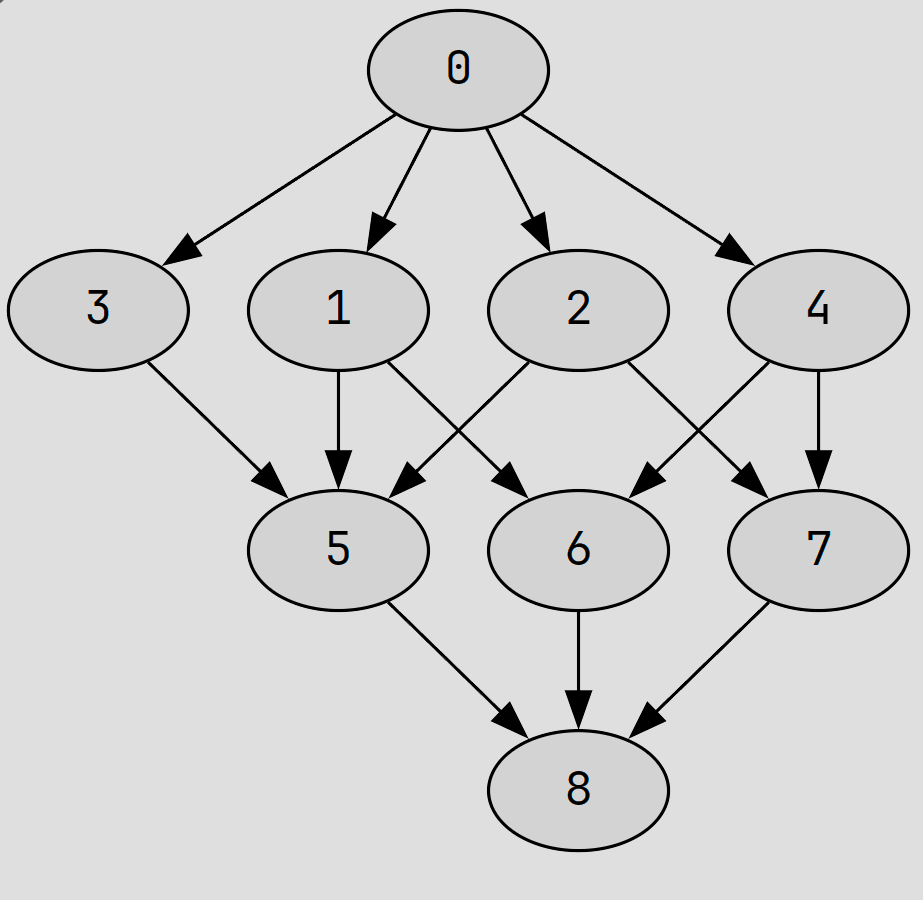
\includegraphics[width=0.40\textwidth]{HEFT_Orthogonal}
            \bicaption{\quad HEFT原文\citep{topcuoglu_performance-effective_2002}示例计算图}
            {\quad Example DAG from HEFT\citep{topcuoglu_performance-effective_2002}}
            \label{fig:HEFT_Orthogonal}
        \end{figure}
        \begin{figure}[!htbp]
            \centering
            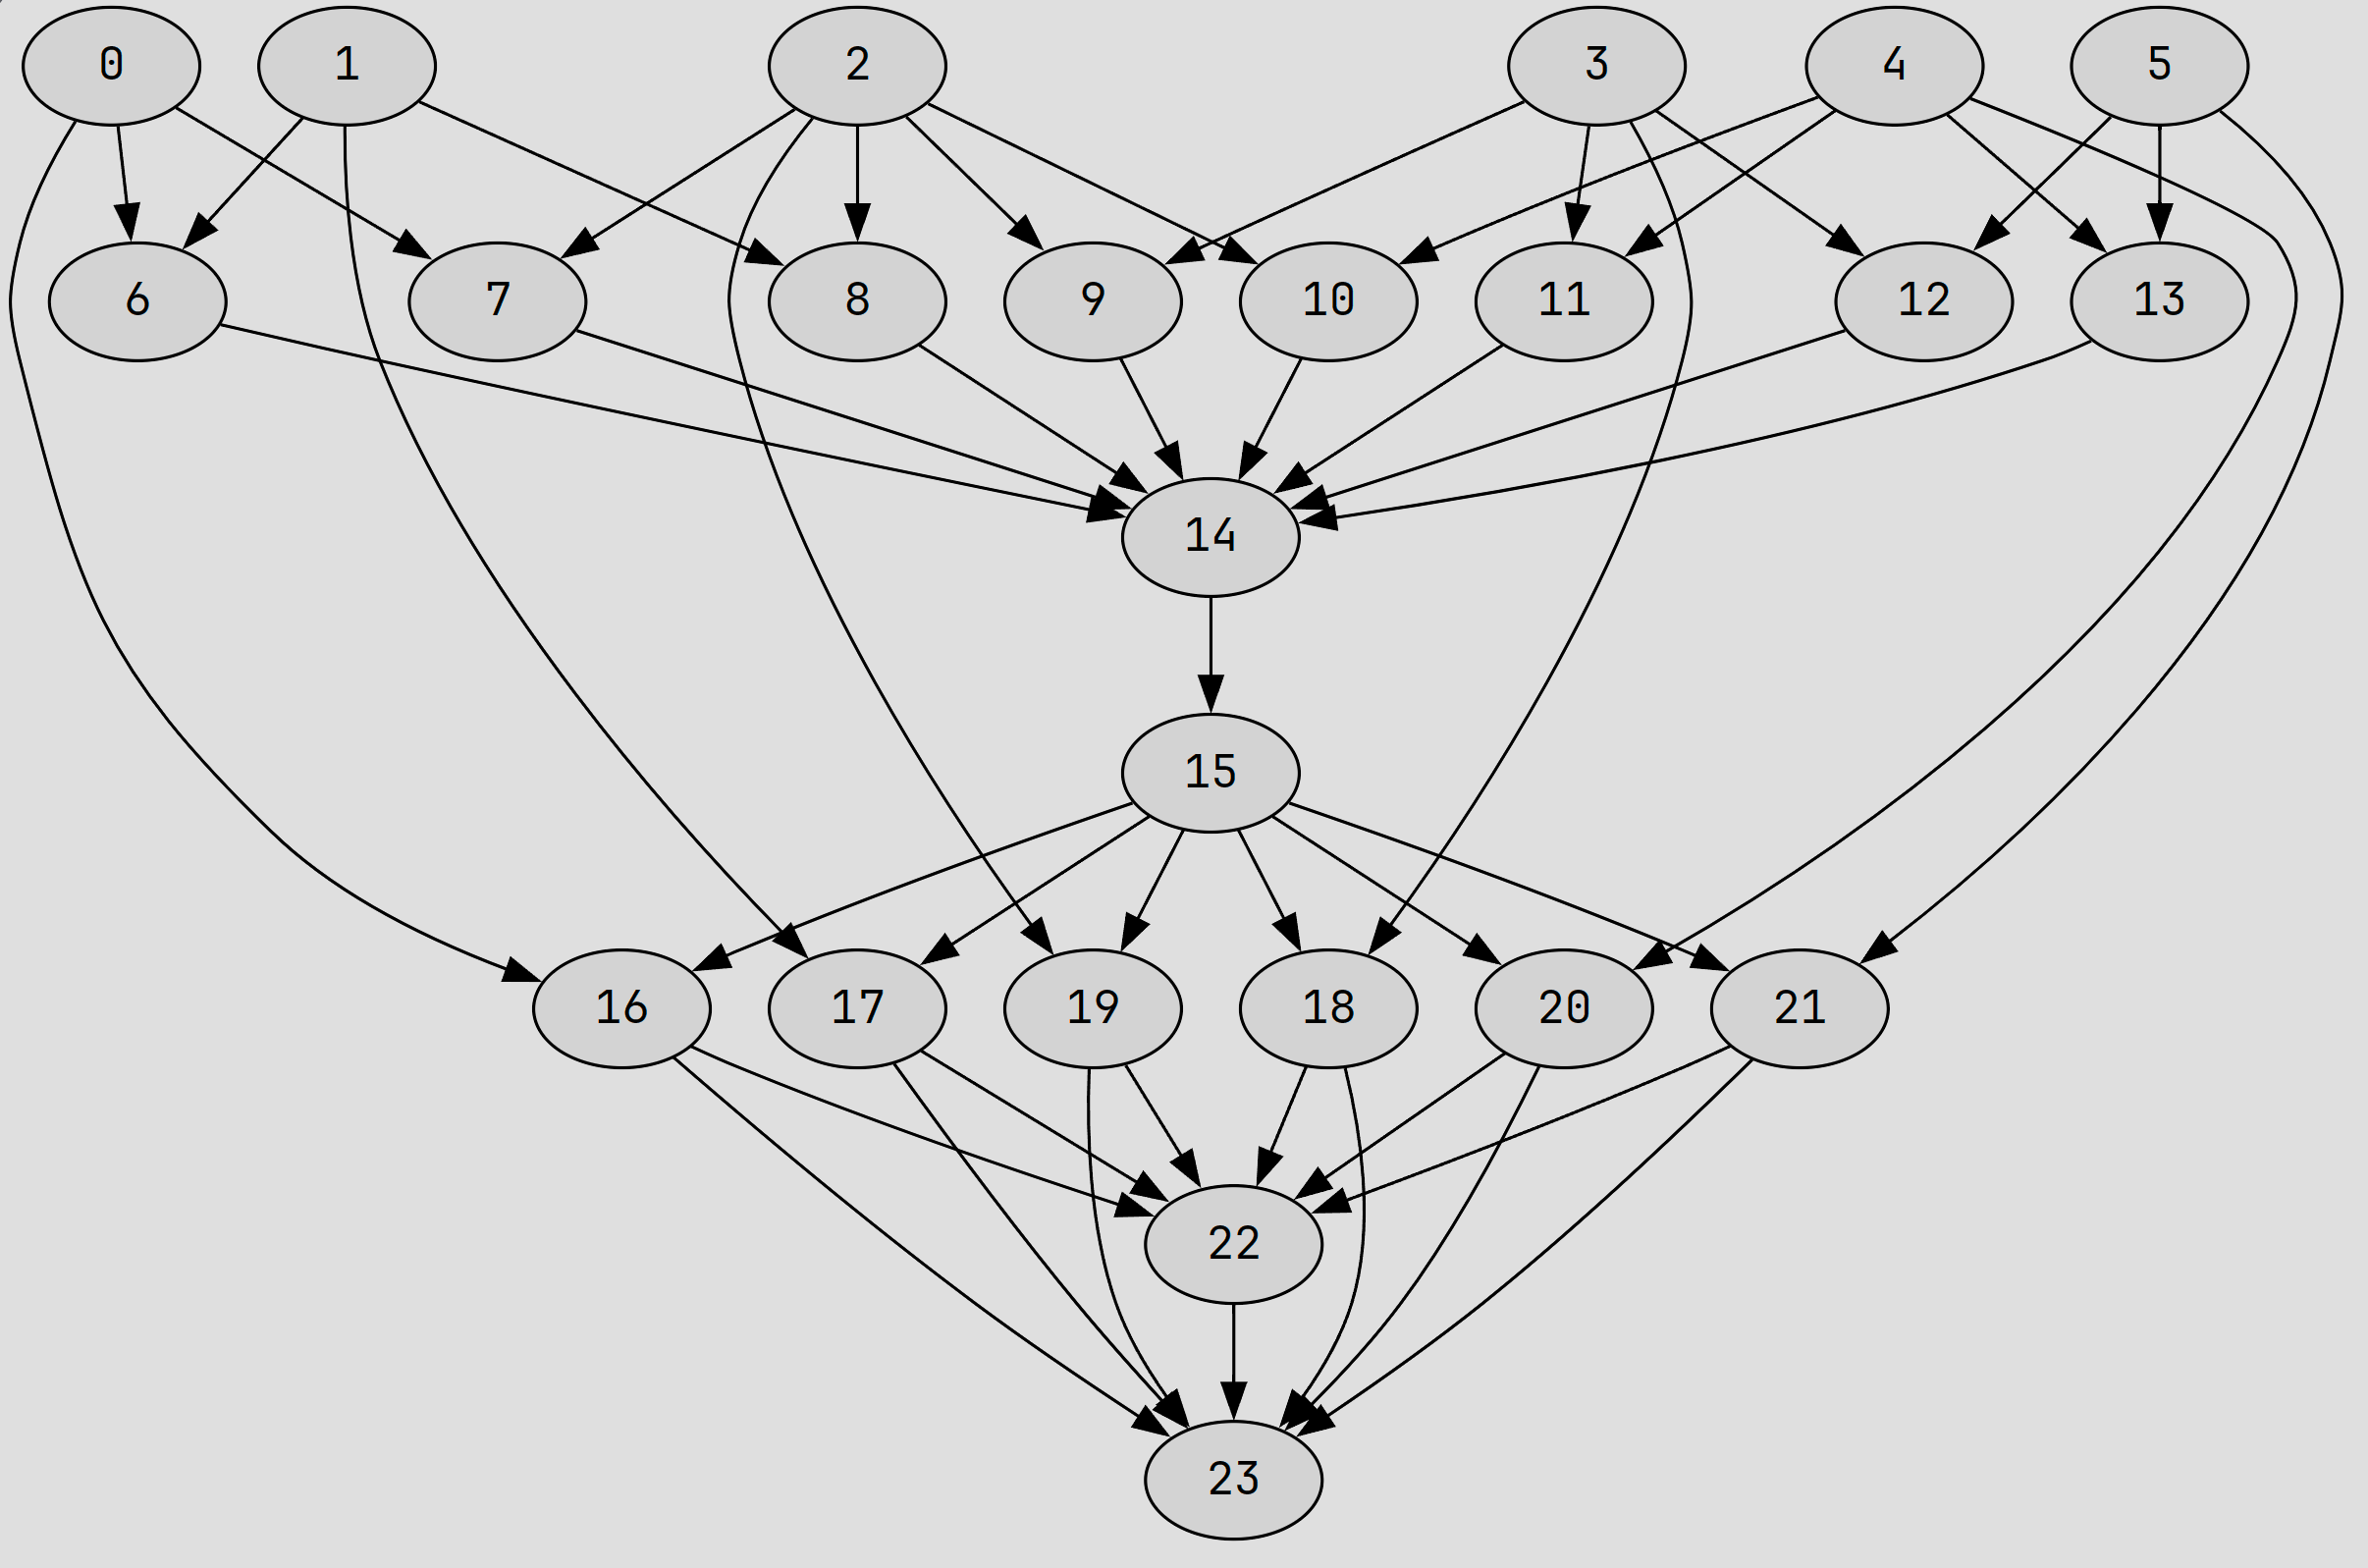
\includegraphics[width=0.85\textwidth]{Montage}
            \bicaption{\quad Montage\citep{deelman_pegasus_2005}计算图}
            {\quad DAG Montage from Pegasus\citep{deelman_pegasus_2005} framework}
            \label{fig:Montage}
        \end{figure}
        
        \subsubsection{随机负载生成算法与混合负载集合}\label{subsec:actual_load_set}
        为了模拟不同现实运行的混合负载,本课题使用了一种随机计算图生成方法。
        该算法将为指定拓扑结构的计算图中的所有结点,按照给定的比例指派访存/计算密集型算子,
        随后为计算图中的所有边指定数据依赖与逻辑依赖。
        
        该算法接受一张制定好节点拓扑结构和数据规模的有向无环图(DAG)
        首先确定DAG中出度为0的节点为终止任务,如果有多个终止任务,则效仿HEFT,加入一个唯一的虚拟终止结点,使原有终止任务与该虚拟节点进行代价为0的逻辑连接。
        对结点集合中节点的属性,采用随机数发生器结合指定比例的二项分布,进行唯一确定其计算密集和访存密集性。
        对边集合中的有向边,采用伯努利分布指定其属性,从而确定数据依赖或逻辑依赖。
        最后对各个确定好属性的结点指定算子类型,已完成最后计算图的构造。

        测试用例的构造中使用了~\ref{subsec:operator_set}中的4中算子以及~\ref{subsec:compute_graph_set}中的两种常用与benchmark的计算图拓扑,生成时选用了20\%, 50\%, 80\%三种不同的访存密集型负载比例,用于模拟不同类型的混合负载。
        %组图:两行(两种拓扑)三列(三种负载比例)
        其中,测试用例的命名方法为“拓扑结构首字母-访存密集型算子占比”,例如M-80则代表含有80\%访存密集型负载的Montage计算图用例,为了便于展示有关于调度具体的细节,本验证将选取某一次随机生成的静态计算图进行展示以及后续评价。有关调度稳定性和调度算法开销的统计分析将被在~\ref{sec:result_analysis}节的最后进行单独叙述。

    \subsection{实验评价指标}\label{sec:evaluation_metrics}
    \textbf{回归模型拟合情况}
    
    对于不同算子在不同输入规模下的运行时性能与能耗,回归模型的拟合效果会直接影响到调度评估时,对性能、能耗数据进行预测的准确性。
    
    \textbf{元启发算法收敛情况}

    不同的元启发算法面对不同的搜索任务时,收敛速度和最终搜索结果的质量会有所差异,元启发算法收敛越快、最优点质量越好,获得的调度性能(或能效比)就越高。
    
    \textbf{整体总线传输量}

    由于调度优化器在优化时将传输所带来的时间和能量开销统计在内,经优化后后所获得的调度策略会尽可能避免非必要的数据搬移,对于整体总线数据传输量的对比也能从一方面展示各种调度策略的质量。
    
    \textbf{整体性能}

    在运行整个包含混合负载的计算图时的时间消耗,用于评价调度所带来的性能变化

    
    \textbf{整体能效比}

    在运行整个包含混合负载的计算图是的时间消耗/能量消耗之比,用于评价调度所带来的能耗比变化。

\section{验证结果与数据分析}\label{sec:experiment_result}
    \subsection{量化数据回归拟合结果}\label{subsec:quantified_regression_training}
    %组图:四算子CPU+DPU性能-规模拟合曲线-残差图
    \begin{figure}[!htbp]
        \centering
        \includegraphics[width=0.85\textwidth]{paper/Img/diagrams/xx}
        \bicaption{\quad }
        {\quad }
        \label{fig:xx}
    \end{figure}
    %组图:四算子CPU+DPU能耗-规模拟合曲线-残差图
    \begin{figure}[!htbp]
        \centering
        \includegraphics[width=0.85\textwidth]{paper/Img/diagrams/xx}
        \bicaption{\quad }
        {\quad }
        \label{fig:xx}
    \end{figure}
    \subsection{元启发算法收敛结果}\label{subsec:metaheuristic_convergence}
    %大型组图:3种元启发算法、3种调度权重下6种示例负载的收敛曲线
    \begin{figure}[!htbp]
        \centering
        \includegraphics[width=0.85\textwidth]{paper/Img/diagrams/xx}
        \bicaption{\quad }
        {\quad }
        \label{fig:xx}
    \end{figure}
    %数据表:3种元启发算法、3种调度权重下6种示例负载最终结果的价值数据、收敛时间和最终选用策略
    \subsection{调度策略及调度结果}\label{subsec:strategies_and_schedules}
    %大型组图:六类调度方法下的最终调度结果
    \begin{figure}[!htbp]
        \centering
        \includegraphics[width=0.85\textwidth]{paper/Img/diagrams/xx}
        \bicaption{\quad }
        {\quad }
        \label{fig:xx}
    \end{figure}
    \subsection{负载执行情况量化评估}\label{subsec:quantified_comparison}
    %大型横图:六类调度方法下的整体性能-能耗-总线传输量的对比,作为最终总结
    \begin{figure}[!htbp]
        \centering
        \includegraphics[width=0.85\textwidth]{paper/Img/diagrams/xx}
        \bicaption{\quad }
        {\quad }
        \label{fig:xx}
    \end{figure}

    \subsection{调度稳定性和开销评估}\label{subsec:scheduling_stability_and_costs_analysis}
    %数据表:使用整个算法进行若干次调度的性能-能耗均值、方差和耗时。

\section{本章小结}\label{sec:RAA_summary}

